% THIS IS SIGPROC-SP.TEX - VERSION 3.1
% WORKS WITH V3.2SP OF ACM_PROC_ARTICLE-SP.CLS
% APRIL 2009
%
% It is an example file showing how to use the 'acm_proc_article-sp.cls' V3.2SP
% LaTeX2e document class file for Conference Proceedings submissions.
% ----------------------------------------------------------------------------------------------------------------
% This .tex file (and associated .cls V3.2SP) *DOES NOT* produce:
%       1) The Permission Statement
%       2) The Conference (location) Info information
%       3) The Copyright Line with ACM data
%       4) Page numbering
% ---------------------------------------------------------------------------------------------------------------
% It is an example which *does* use the .bib file (from which the .bbl file
% is produced).
% REMEMBER HOWEVER: After having produced the .bbl file,
% and prior to final submission,
% you need to 'insert'  your .bbl file into your source .tex file so as to provide
% ONE 'self-contained' source file.
%
% Questions regarding SIGS should be sent to
% Adrienne Griscti ---> griscti@acm.org
%
% Questions/suggestions regarding the guidelines, .tex and .cls files, etc. to
% Gerald Murray ---> murray@hq.acm.org
%
% For tracking purposes - this is V3.1SP - APRIL 2009

\documentclass{acm_proc_article-sp}

\usepackage{booktabs}

\usepackage{fontspec}

\usepackage{polyglossia}
\setmainlanguage{brazil}

\usepackage{graphicx}
\DeclareGraphicsExtensions{.pdf,.png,.jpg}
\graphicspath{{./img/}}

\usepackage{verbatim}
\usepackage{hyperref}

\usepackage[backend=biber,style=numeric,citestyle=numeric]{biblatex}
\addbibresource{references.bib}

\usepackage[table]{xcolor}
\usepackage{booktabs}

\usepackage{afterpage}

\begin{document}

\title{Seleção de Atributos para Analise de Agrupamento de Dados}
\subtitle{Um Estudo Comparativo} 
%\titlenote{A full version of this paper is available as
%\textit{Author's Guide to Preparing ACM SIG Proceedings Using
%\LaTeX$2_\epsilon$\ and BibTeX} at
%\texttt{www.acm.org/eaddress.htm}}}
%
% You need the command \numberofauthors to handle the 'placement
% and alignment' of the authors beneath the title.
%
% For aesthetic reasons, we recommend 'three authors at a time'
% i.e. three 'name/affiliation blocks' be placed beneath the title.
%
% NOTE: You are NOT restricted in how many 'rows' of
% "name/affiliations" may appear. We just ask that you restrict
% the number of 'columns' to three.
%
% Because of the available 'opening page real-estate'
% we ask you to refrain from putting more than six authors
% (two rows with three columns) beneath the article title.
% More than six makes the first-page appear very cluttered indeed.
%
% Use the \alignauthor commands to handle the names
% and affiliations for an 'aesthetic maximum' of six authors.
% Add names, affiliations, addresses for
% the seventh etc. author(s) as the argument for the
% \additionalauthors command.
% These 'additional authors' will be output/set for you
% without further effort on your part as the last section in
% the body of your article BEFORE References or any Appendices.

\numberofauthors{1} %  in this sample file, there are a *total*
% of EIGHT authors. SIX appear on the 'first-page' (for formatting
% reasons) and the remaining two appear in the \additionalauthors section.
%
\author{
% You can go ahead and credit any number of authors here,
% e.g. one 'row of three' or two rows (consisting of one row of three
% and a second row of one, two or three).
%
% The command \alignauthor (no curly braces needed) should
% precede each author name, affiliation/snail-mail address and
% e-mail address. Additionally, tag each line of
% affiliation/address with \affaddr, and tag the
% e-mail address with \email.
%
% 1st. author
\alignauthor
Sibelius Seraphini\\
    \affaddr{Instituto de Ciências Matemáticas e de Computação (ICMC) - Universidade de São Paulo (USP)}\\
    \affaddr{Avenida Trabalhador São-carlense, 400 - Centro}
    \affaddr{São Carlos, Brasil}
    \email{sibelius@usp.br}
}
% There's nothing stopping you putting the seventh, eighth, etc.
% author on the opening page (as the 'third row') but we ask,
% for aesthetic reasons that you place these 'additional authors'
% in the \additional authors block, viz.
% Just remember to make sure that the TOTAL number of authors
% is the number that will appear on the first page PLUS the
% number that will appear in the \additionalauthors section.

\maketitle
\begin{abstract}
% 200 to 300 words
% Components of an abstract
% 1. Motivation or Statement of Problem: Why do we care about the problem? What practical, theoretical, scientific, or artistic gap is your research filling?
% 2. Methods or Approach: What did you actually do to get your results? Did you analyze three plays, interview 125 students, write a memoir, invent a more powerful photovoltaic cell, or translate a book? Did you approach your subject using a specific theoretical framework, technical procedure, or methodology?
% 3. Results or Product: As a result of completing the above procedure or investigation, what did you learn, create, or invent?
% 4. Conclusions or Implications: What are the larger implications of your findings, especially for the problem or gap identified in Step 1?
O objetivo da seleção de atributos para aprendizado não-supervisionado é encontrar o menor subconjunto de atributos que melhor revela agrupamentos naturais interessantes.
O problema se torna ainda mais complexo se o número de agrupamento não é conhecido.
Consequentemente, existe a necessidade de encontrar o número de grupos concomitantemente com o subconjunto de atributos, que geralmente são inter-relacionados.
Na literatura existem alguns trabalhos que propõem algoritmos para seleção de atributos para agrupamento de dados.
Desse modo, este artigo visa realizar um estudo comparativo entre alguns dos algoritmos propostos na literatura, com o objetivo de identificar qual deles é melhor para um determinado cenário.
Os algoritmos foram aplicados sistematicamente em conjuntos de dados gerados segundo um design fatorial experimental.
Dois critérios de validação externa foram utilizado para o realizar o comparativo entre os algoritmos.
Três aspectos foram levados em conta para avaliar os algoritmos: qualidade do agrupamento obtido (critério externo), estimativa do número de agrupamentos, e quantidade de atributos selecionados.
Os algoritmos \textit{clustvarsel} e \textit{vscc} apresentaram os melhores resultados, não apresentando diferença estatisticamente significativas entre si.
A ampliação do conjunto de dados sinteticos e a acréscimo de outros conjuntos de dados reais podem constituir um benchmark para novos algoritmos de seleção de atributos para agrupamento de dados.


\end{abstract}

% A category with the (minimum) three required fields
%\category{H.4}{Information Systems Applications}{Miscellaneous}
%A category including the fourth, optional field follows...
%\category{D.2.8}{Software Engineering}{Metrics}[complexity measures, performance measures]

%\terms{Theory}

%\keywords{ACM proceedings, \LaTeX, text tagging} % NOT required for Proceedings

\section{Introdução}
% Contextualization and Motivation
% Aims (Goals) of this paper
% Following sections organization

% why do feature selection ?
% why is it harder for clustering problems?
% 
% explain feature selection
% explain feature selection challenges for clustering problems
% explain clustering

%1. improve clustering performance
%2. improve understanding of the model
%3. remove noisy variables, to help the distinction of groups
O agrupamento de dados é um problema fundamental na mineração de dados, em que se visa determinar um conjunto finito de categorias para descrever um conjunto de dados de acordo com as similaridades entre os seus objetos~\cite{jain1988algorithms, kaufman2009finding, everitt2001clustering, gan2007data}
Nesse problema, a estrutura de maior interesse para o investigador pode ser melhor representada usando apenas alguns dos atributos.
Além disso, utilizando-se somente os atributos relevantes do conjunto de dados pode levar a um melhor modelo de agrupamento de dados para descrever os dados futuros, e também menos atributos podem produzir uma melhor partição de dados em grupos mais próximos da estrutura dos grupos verdadeiros.
Nesse sentido, uma tarefa importante de analise estatística e mineração de dados é a seleção de atributos.
A seleção de atributos visa escolher um subconjunto dos atributos originais, eliminando os redundantes, não informativos, e ruidosos.
Existem vários potencias benefícios da seleção de atributos como, por exemplo~\cite{guyon2003introduction}: facilitar o entendimento e visualização dos dados, reduzir as necessidades de medição e armazenamento, reduzir o tempo de treinamento e utilização e diminuir a maldição da dimensionalidade para melhorar o desempenho de predição.

A literatura para seleção de atributos para classificação (aprendizado supervisionado) é vasta~\cite{dash1997feature, fukunaga1990introduction, almuallim1991learning, kohavi1997wrappers}.
Para o aprendizado supervisionado, os algoritmos de seleção de atributos maximizam alguma função de capacidade preditiva.
Porque são dados as classes dos objetos, é natural manter somente os atributos que são relacionados com essas classes.
Mas no caso do aprendizado não-supervisionado, não se conhece a priori as classes (grupos) dos objetos.
Além disso, o problema se torna ainda mais complexo se o número de grupos da base de dados não é conhecido a priori.
Consequentemente, existe a necessidade de encontrar o número de grupos concomitantemente com o subconjunto de atributos, que geralmente são inter-relacionados.

% Aims of this paper
% make a comparison of different feature selection algorithms for clustering
Levando isto em consideração, este artigo visa realizar um estudo comparativo de alguns algoritmos de seleção de atributos para agrupamento de dados.
Esse estudo tem dois objetivos: o primeiro é verificar se a seleção de atributos melhora o modelo de agrupamento de dados; o segundo é identificar qual dos algoritmos investigados melhor consegue identificar atributos relevantes, melhorando assim o agrupamento de dados. 
Desse modo, dois algoritmos de agrupamentos serão treinados utilizando todos os atributos, k-means~\cite{hartigan1979algorithm, macqueen1967some} e EM ou baseado em modelo~\cite{fraley2002model, dempster1977maximum,hastie2009elements}.
Ademais, quatro algoritmos de seleção de atributos: sparse K-means~\cite{witten2010framework, macqueen1967some}, clustvarsel~\cite{raftery2006variable}, vscc~\cite{andrews2013variable}, baseado na silhueta simplificada (SS)~\cite{hruschka2005feature}; serão utilizados para selecionar os atributos relevantes, após os algoritmos k-means e EM serão treinados utilizando o subconjunto de atributos selecionados.
A comparação entre o grupo que considera todos os atributos e o que considera os atributos selecionados, assim como a comparação entre os algoritmos de seleção de atributos investigados será feita utilizando dois critérios de validação externa: índice de Rand ajustado~\cite{hubert1985comparing} e Jaccard~\cite{jain1988algorithms}.
% também se levará em consideração a taxa de erro de classificação (CER --- \textit{classification error rate}).

O restante desse artigo é estruturado como segue.
A Seção~\ref{sec:relatedwork} apresenta o conceito da seleção de atributos e os algoritmos de seleção de atributos para agrupamento de dados que serão investigados nesse estudo comparativo.
Além disso, também descreve sobre critérios de validação de agrupamento e em particular sobre os dois critérios que serão empregadas nesse estudo comparativo.
Na Seção~\ref{sec:experiments} é descrito os conjuntos de dados utilizados, assim como a metodologia empregada e também apresenta-se os resultados e discussões.
Finalmente, a Seção~\ref{sec:conclusions} aborda as conclusões desse estudo comparativo.

\section{Trabalhos Relacionados}
\label{sec:relatedwork}
% External validity index (adjusted Rand Index, Jaccard, classification error)
% feature selection algorithms (k-means, modelbased (em), sparseKmeans, clustvarsel, vscc, simplifiedSilhouette)

\subsection{Seleção de Atributos para Agrupamento de Dados}

O objetivo da seleção de atributos para aprendizado não-supervisionado é encontrar o menor subconjunto de atributos que melhor revela agrupamentos naturais interessantes (grupos)~\cite{dy2004feature}.
Os métodos de seleção de atributos são classificados em três tipos:
\begin{itemize}
    \item \textit{abordagem de filtro}: atributos são avaliados individualmente usando o objetivo da tarefa e um valor de relevância é calculado que é utilizado para ordenar os atributos
    \item \textit{abordagem wrapper}: atributos são avaliados num subconjunto, um algoritmo que realiza a tarefa de aprendizado é utilizado para essa avaliação
    \item \textit{abordagem embutida}: a seleção dos atributos mais importantes é parte integrada do tarefa de aprendizado
\end{itemize}

Um algoritmo que utilizado a abordagem \textit{wrapper} é o proposto por~\cite{hruschka2005feature}.
\cite{hruschka2005feature} apresenta um algoritmo que não necessita do número de grupos a priori, encontrando tanto o número de grupos e o subconjunto de atributos que exibe o maior valor de silhueta simplificada~\cite{hruschka2005feature}, critério de validação interna.
O algoritmo emprega a busca sequencial \textit{forward search}~\cite{liu2005toward}, que começa com um subconjunto vazio e sucessivamente adiciona atributos; o algoritmo k-means em conjunto com o critério silhueta simplificada é utilizado para avaliar o subconjunto de atributos. 

Em contrapartida,~\cite{witten2010framework} modela o problema de seleção de atributos como um problema de otimização, no qual cada atributo possui um peso.
Nessa abordagem, os atributos selecionados são aqueles que apresentam peso diferente de zero, após o problema ser maximizado. 

Outra técnica de seleção de atributos é dada por~\cite{raftery2006variable}, onde múltiplos modelos da família MCLUST são comparados usando fatores aproximados de Bayes~\cite{kass1995bayes}.
Essa técnica encontra-se disponível no pacote \textit{clustvarsel}~\cite{dean2006clustvarsel} do \textit{R}.
Contudo, por causa do número de parâmetros que exige estimativa de alguns modelos \textit{mclust} é quadrático na dimensionalidade dos dados, o pacote \textit{clustvarsel} pode ser muito lento em grandes dimensões.
Além disso, essa técnica às vezes pode levar a resultados inferiores quando comparados com o uso de \textit{mclust} sozinho~\cite{mcnicholas2008parsimonious}

Além disso,~\cite{andrews2013variable} introduz uma técnica de seleção de atributos que é intuitiva e computacionalmente eficiente, podendo ser utilizada tanto para problemas de agrupamento de dados como classificação.
O método proposto consiste em definir uma relação entre a variância entre grupos e a correlação entre as variáveis.
Cinco relações foram escolhidas para selecionar os subconjuntos de atributos.
Os subconjuntos são avaliados utilizando o critério de informação Bayesiana (BIC)~\cite{schwarz1978estimating}, que mede o grau de incerteza do modelo. 

\subsection{Critérios de Validação Externos}
\label{sec:external_criterion}
Índices ou Critérios de validação de agrupamento~\cite{halkidi2001clustering, milligan1985examination} são usados para avaliar a validade das partições obtidas por um algoritmo de agrupamento pela comparação de suas características com uma referencia ou partição ideal.
Esses índices calculam um valor relativo ou absoluto para a semelhança entre as diferentes partições dos mesmos dados.

Esses índices podem ser classificados em critérios externos, internos e relativos.
Os primeiros assumem que a avaliação da partição é baseada em uma estrutura pré-especificada que reflete a estrutura natural do conjunto de dados.
Para os segundos, a avaliação é realizada em termos de quantidades obtidas a partir dos valores dos atributos que descrevem os grupos, que medem quão separados e compactos são.
Os últimos assumem que é realizado uma comparação entre uma partição com outras obtidas utilizando diferentes parâmetros do algoritmo de agrupamento de dados ou outro algoritmo de agrupamento.
Geralmente são critérios internos capazes de quantificar a qualidade de agrupamentos.

A ideia principal dos critérios externos é que quando dois exemplos pertencem a um grupo natural nos dados, eles usualmente aparecem no mesmo grupo quando diferentes partições são obtidas.
Isso significa que duas partições que mantêm essas coassociações são mais similares e representam uma estrutura similar para o conjunto de dados.
Para calcular esses índices, a coincidência de cada par de exemplos nos grupos de dois agrupamentos tem de ser contado, existem quatro possíveis casos:
\begin{itemize}
    \item \textit{a}: Número de pares de objetos de dados que pertencem a mesma classe em C e ao mesmo grupo em P.
    \item \textit{b}: Número de pares de objetos de dados que pertencem a mesma classe em C e a diferente grupos em P.
    \item \textit{c}: Número de pares de objetos de dados que pertencem a diferentes classes em C e ao mesmo grupo em P.  
    \item \textit{d}: Número de pares de objetos de dados que pertencem a diferentes classes em C e a diferente grupos em P.
\end{itemize}  

Destes valores diferentes índices de similaridade podem ser definidos para comparação de duas partições:
\begin{itemize}
    \item \textit{Adjusted Rand Index (ARI)}~\cite{hubert1985comparing,jain1988algorithms}:
$$ AR = \frac{a - \frac{(a+c)(a+b)}{a+b+c+d}}{\frac{(a+c)+(a+b)}{2} - \frac{(a+c)(b+c)}{a+b+c+d}} $$

    \item \textit{Jaccard Coeffient}~\cite{jain1988algorithms,kaufman2009finding}:
$$ J = \frac{a}{a+b+c} $$
\end{itemize}

Os dois critérios de validação externos apresentados serão utilizados na metodologia proposta para comparar os algoritmos de seleção de atributos.
A próxima Seção descreve a metodologia para realizar este estudo comparativo.

\begin{table*}
    \centering
    \begin{tabular}{ccccccc}
        \toprule
        & Grupos & Separação & Atributos & \multicolumn{1}{p{1.5cm}}{Atributos Ruidosos} & Réplicas\\
        \midrule
        Fatores & 2, 3, 5   & L, M, H   & 2, 5, 10  & 0, 1, 3, 10   & 1,2,3     & Total\\
        \midrule
        Níveis & 3          & 3         & 3         & 4             & 3         & 324\\
       % \midrule
       % Total & 324 \\
        \bottomrule
    \end{tabular}
    \caption{Característica do design fatorial experimental utilizado para gerar os conjuntos de dados}
    \label{tab:datasets}
\end{table*}

\section{Experimentos}
\label{sec:experiments}

\subsection{Conjuntos de Dados}
\label{sec:datasets}
% factorial design (clustGeneration)
Para comparar os algoritmos de seleção de atributos para agrupamento de dados utilizou-se um conjunto de dados sintéticos.
Os conjuntos de dados foram gerados utilizando o pacote \textit{clusterGeneration} que implementa a metodologia descrita em~\cite{qiu2006generation}.
A Tabela~\ref{tab:datasets} apresenta o fatores de design experimental para gerar os conjuntos de dados.
A geração utilizou-se de quatro fatores de design: grupos --- define o número de agrupamentos; separação, L --- agrupamento próximo, M --- agrupamento separado, H --- agrupamento bem separado; atributos --- atributos relevantes; atributos ruidosos --- atributos que não trazer informações sobre o agrupamento.
Em resumo, os quatro fatores de design experimental descritos acima foram combinados, assim produzindo um conjunto de 108 (3 número de agrupamentos x 3 graus de separabilidade x 3 números de atributos x 4 números de atributos ruidosos). 
Seguindo o design de~\cite{milligan1985examination} e para obter uma melhor confiança estatística, três replicações independentes foram utilizadas para cada combinação, logo, resultando em 324 conjuntos de dados.
    
\subsection{Metodologia Experimental}
% sample distributions hardly satisfy the normality assumption.
% Wilcoxon/Mann-Whitney (W/M-W) test
% The efficiency of the W/M-W test is 0.95 with respect to parametric tests like the t-test or the z-test even if the data are normal. Thus, even when the normality assump- tion is satisfied, the W/M-W test might be preferred \cite{triola2006elementary}
Com os conjuntos de dados gerados, dois algoritmos de agrupamentos de dados e quatro algoritmos de seleção de atributos para agrupamento de dados, i.e., k-means~\cite{hartigan1979algorithm,macqueen1967some} e EM~\cite{fraley2002model,dempster1977maximum,hastie2009elements}; e sparse K-means~\cite{witten2010framework}, clustvarsel~\cite{raftery2006variable}, vscc~\cite{andrews2013variable}, baseado na silhueta simplificada (SS)~\cite{hruschka2005feature}, foram sistematicamente aplicados para cada conjunto de dados. 
Os algoritmos k-means e EM utilizam todos os atributos do conjunto de dados.
Dentre os algoritmos de seleção de atributos, somente o sparse K-means exige que o número de agrupamento seja fornecido a priori.
Nesse sentido, conduziu-se dois experimentos: o primeiro aplica todos os algoritmos acima fornecendo o número de agrupamentos verdadeiros; no segundo aplicou-se somente os algoritmos \textit{clustvarsel} e \textit{vscc}\footnote{O algoritmo \textit{SS} não foi empregado por não ser computacionalmene eficient}, sem que o número de agrupamentos verdadeiros fossem fornecidos.
Devido a isso, o primeiro experimento aplica todos os algoritmos acima fornecendo o número de agrupamentos a priori, para que fosse possível o comparativo entre eles.

Para melhorar confiança da analise, os resultados correspondem a dois critérios de validação externos distintos descritos na Seção~\ref{sec:external_criterion}, i.e., ARI e coeficiente Jaccard.
Histogramas dos resultados sugerem fortemente que as distribuições amostrais observados dificilmente satisfazem a suposição de normalidade.
Por essa razão, será adotado o teste não-parametrico de Wilcoxon/Mann-Whitney (W/M-W)
A eficiência do teste W/M-W é 0.95 com relação a testes paramétricos como o teste T ou o teste Z mesmo se os dados são normais.
Assim, mesmo quando a suposição de normalidade é satisfeito, o teste W/M-W pode ser preferível~\cite{triola2006elementary}.
Esse teste será usado nesse trabalho para comparar o resultado de cada par de algoritmos como duas amostras.

Ademais, para o segundo experimento, o número de agrupamentos de uma partição eleita como a melhor pelo algoritmo de seleção de atributos é comparado contra o número certo de agrupamentos conhecido para um conjunto de dados particular.
O maior número de acertos é 324 (número de conjuntos de dados).

\begin{table}
    \centering
    \begin{tabular}{ccc}
        \toprule
        Algoritmo & Nº de Acertos & \% \\
        \midrule
        clustvarsel & 304 & 93.82 \\
        vscc        & 303 & 93.51 \\
        \bottomrule
    \end{tabular}
    \caption{Número de acertos de estimativa do número de agrupamentos para cada algoritmo considerando uma coleção de 324 conjuntos de dados\protect\footnotemark}
    \label{tab:hits}
\end{table}

\subsection{Resultados Experimental}
\label{sec:results}

A Tabela~\ref{tab:hits} mostra o número de acertos e a porcentagem para o número correto de agrupamentos.
Portanto, tanto o algoritmo \textit{clustvarsel} e \textit{vscc} conseguem estimar bem o número correto de agrupamentos (93\%)
A média de número de acertos dos grupos \textit{clustvarsel} e \textit{vscc} são 0.938 e 0.935; as distribuições nos dois grupos não difere significativamente (Mann–Whitney U = 52650, n1 = n2 = 324, P = 0.436 unicaudal).

Os resultados do primeiro experimento utilizando o critério externo ARI é reportado na Tabela~\ref{tab:ariMeans}.
As médias dos valores do ARI --- computados sobre toda a coleção de $N_{D}=324$ valores disponíveis (um para cada conjunto de dados) --- é apresentado na parte inferior da tabela.
Os valores mostrados em cada celula do topo da tabela correspondem a diferença entre as médias dos correspondentes pares de algoritmos.
Uma célula sombreado indica que a correspondente diferença é estatisticamente significante para nível de $\alpha=5\%$ (teste unicaudal) com relação ao teste W/M-W.

Vale lembrar que a analise exemplificada na Tabela~\ref{tab:ariMeans} também foi realizada para o critério externo Jaccard (Apêndice, Tabela~\ref{tab:jaccardMeans}).
Levando em consideração ambas as tabelas, podemos derivar algumas conclusões interessantes.
Os algoritmos \textit{clustvarsel}, \textit{EM}, \textit{vscc} apresentam resultados melhores do que os outros algoritmos, porém não apresentam diferenças significativas entre si. 
O algoritmo baseado na silhueta simplificada apresenta o pior resultado entre os algoritmos.

Ademais, buscou-se verificar se os algoritmos conseguiram eliminar os atributos ruidosos.
A Figura~\ref{fig:subsets} apresenta um gráfico boxplot com os valores do tamanho do subconjunto de atributos que foram selecionados por cada algoritmo.
Vale destacar, que o boxplot rosa, roxo e marrom correspondem aos valores dos atributos ruidosos, dos atributos não-ruidosos, e do total de atributos, respectivamente.
A partir desse gráfico, verificamos que o algoritmo sparseKmeans seleciona praticamente todos os atributos, porém como ele atribui um peso para cada atributo, mesmo atributos com pesos próximo de zero são considerados como selecionados.
Por outro lado, o algoritmo baseado em silhueta simplifica seleciona poucos atributos, perdendo informações importantes dos outros atributos para encontrar os agrupamentos.
Tanto o \textit{clustvarsel} quanto o \textit{vscc} conseguem eliminar os atributos ruidosos, chegando mais perto do subconjunto contendo somente os atributos relevantes.

Levando em consideração as três analises realizadas nesse estudo comparativo, pode-se derivar que dentre os algoritmos de seleção de atributos investigados os que obtiveram os melhores resultados foram os \textit{clustvarsel} e \textit{vscc}.
Ambos conseguem identificar o correto número de agrupamentos (~93\% de acerto nos conjuntos de dados), também apresentam um resultado superior aos outros algoritmos considerando-se os dois critérios de validação externos utilizados.
Além disso, também conseguem eliminar razoavelmente os atributos irrelevantes.

\begin{figure}
    \centering
    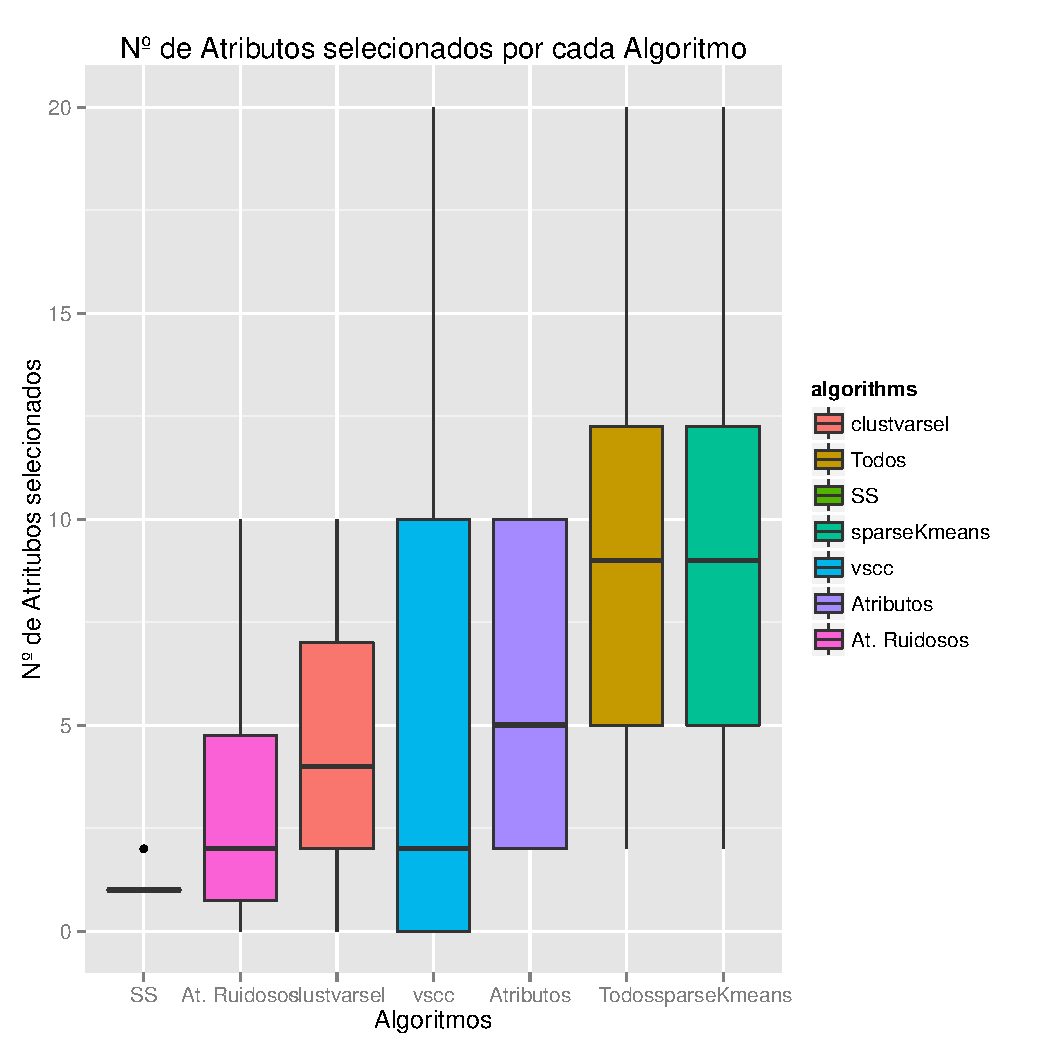
\includegraphics[width=0.5\textwidth]{subset}
    \caption{Nº de Atributos selecionados por cada Algoritmo}
    \label{fig:subsets}
\end{figure}

\begin{table*}
    \centering
    \begin{tabular}{cccccccc}
        \toprule
                  & & A & B & C & D & E & F \\
        \midrule
\textit{clustvarsel}     & A &  0.000 & 0.011 & 0.013 & \cellcolor{gray}0.051 &\cellcolor{gray} 0.075 &\cellcolor{gray} 0.319 \\
\textit{EM}              & B & -0.011 & 0.000 & 0.002 & 0.039 &\cellcolor{gray} 0.063 &\cellcolor{gray} 0.307 \\
\textit{vscc}            & C & -0.013 &-0.002 & 0.000 &\cellcolor{gray} 0.037 &\cellcolor{gray} 0.061 &\cellcolor{gray} 0.305 \\
\textit{sparseKmeans}    & D & \cellcolor{gray}-0.051 &-0.039 &\cellcolor{gray}-0.037 & 0.000 & 0.024 &\cellcolor{gray} 0.268 \\
\textit{k-means}         & E & \cellcolor{gray}-0.075 &\cellcolor{gray}-0.063 &\cellcolor{gray}-0.061 &-0.024 & 0.000 &\cellcolor{gray} 0.244 \\
\textit{SS}              & F & \cellcolor{gray}-0.319 &\cellcolor{gray}-0.307 &\cellcolor{gray}-0.305 &\cellcolor{gray}-0.268 &\cellcolor{gray}-0.244 & 0.000 \\ \\
        \midrule
            & mean  &  0.939 & 0.927 & 0.925 & 0.888 & 0.864 & 0.619 \\
        \bottomrule
    \end{tabular}
    \caption{Valores Médios e suas diferenças para o critério externo ARI}
    \label{tab:ariMeans}
\end{table*}

\section{Conclusões e Trabalhos Futuros}
\label{sec:conclusions}

\footnotetext{O algoritmo \textit{sparseKmeans} não estima o número de agrupamentos, e o \textit{SS} não foi empregado por não ser computacionalmente eficiente} 

Esse artigo apresentou um estudo comparativo entre algoritmos de seleção de atributos para agrupamento de dados.
O design fatorial experimental utilizado para gerar os conjuntos de dados produziu 324 conjuntos de dados considerando as replicações para melhorar a confidência estatística.
Dois algoritmos de agrupamento de dados (k-means e EM) e quatro algoritmos de seleção de atributos foram sistematicamente aplicados para conjunto de dados.
O teste de Wilcoxon/Mann-Whitney foi utilizado para testar se as diferenças entre as médias dos critérios externos obtidos pelos algoritmos são diferentes tem significância estatística.  
Três analises foram realizadas: a primeira que verifica se os algoritmos de seleção de atributos apresentam qualidades diferentes de agrupamentos, avaliados pelos dois critérios de validação externa; a segunda que verifica se os algoritmos de seleção de atributos, que não necessitam do número de grupos a priori, conseguem identificar o número corretos de agrupamentos; finalmente, a terceira que verifica se os algoritmos de seleção de atributos conseguem eliminar os atributos ruidosos, selecionando somente os relevantes.
Levando as três analises em consideração, os algoritmos de seleção de atributos que apresentaram os melhores resultados foram o \textit{clustvarsel} e o \textit{vscc}.

Em relação a trabalhos futuros, os conjuntos de dados devem ser aumentados para dados com grandes dimensões, tais como os banco de dados de genes.
Também devem ser aplicados conjuntos de dados reais, para verificar a validade de tais algoritmos.
Assim, os conjuntos de dados sinteticos em conjunto com base de dados reais devem ser utilizados para compor um benchmark para novos algoritmos de seleção de atributos.
Além disso, um número maior de algoritmos de seleção de atributos devem ser considerados. 


%\end{document}  % This is where a 'short' article might terminate

%
% The following two commands are all you need in the
% initial runs of your .tex file to
% produce the bibliography for the citations in your paper.
\printbibliography % biblatex
%\bibliographystyle{abbrv}
%\bibliography{references}  % sigproc.bib is the name of the Bibliography in this case
% You must have a proper ".bib" file
%  and remember to run:
% latex bibtex latex latex
% to resolve all references
%
% ACM needs 'a single self-contained file'!
%

\appendix
O apêndice traz as mesmas informações da Tabela~\ref{tab:ariMeans}, mas para o coeficiente de Jaccard, Tabela~\ref{tab:jaccardMeans}.

\begin{table*}[!t]
    \centering
    \begin{tabular}{cccccccc}
    \toprule
                   &        &  A     &  B    & C     & D     & E     & F \\
\textit{clustvarsel} & A    &  0.000 & 0.011 & 0.008 &\cellcolor{gray} 0.049 &\cellcolor{gray} 0.074 &\cellcolor{gray}0.289 \\
\textit{EM}          & B    & -0.011 & 0.000 &-0.002 & 0.038 &\cellcolor{gray} 0.063 &\cellcolor{gray}0.278 \\
\textit{vscc}        & C    & -0.008 & 0.002 & 0.000 &\cellcolor{gray} 0.041 &\cellcolor{gray} 0.066 &\cellcolor{gray}0.281 \\
\textit{sparseKmeans}& D    &\cellcolor{gray} -0.049 &-0.038 &\cellcolor{gray}-0.041 & 0.000 & 0.025 &\cellcolor{gray}0.239 \\
\textit{k-means}     & E    &\cellcolor{gray} -0.074 &\cellcolor{gray}-0.063 &\cellcolor{gray}-0.066 &-0.025 & 0.000 &\cellcolor{gray}0.214 \\
\textit{SS}          & F    &\cellcolor{gray} -0.289 &\cellcolor{gray}-0.278 &\cellcolor{gray}-0.281 &\cellcolor{gray}-0.239 &\cellcolor{gray}-0.214 &0.000 \\
    \midrule
            & mean      &  0.932 & 0.921 & 0.924 & 0.882 & 0.857 &0.642 \\
    \bottomrule
    \end{tabular}
    \caption{Valores Médios e suas diferenças para o critério externo Jaccard}
    \label{tab:jaccardMeans}
\end{table*}



\balancecolumns
% That's all folks!
\end{document}
